\section{Experiment}
    \subsection{Data Preprocessing}
        \begin{figure}[tbh]
            \centering
            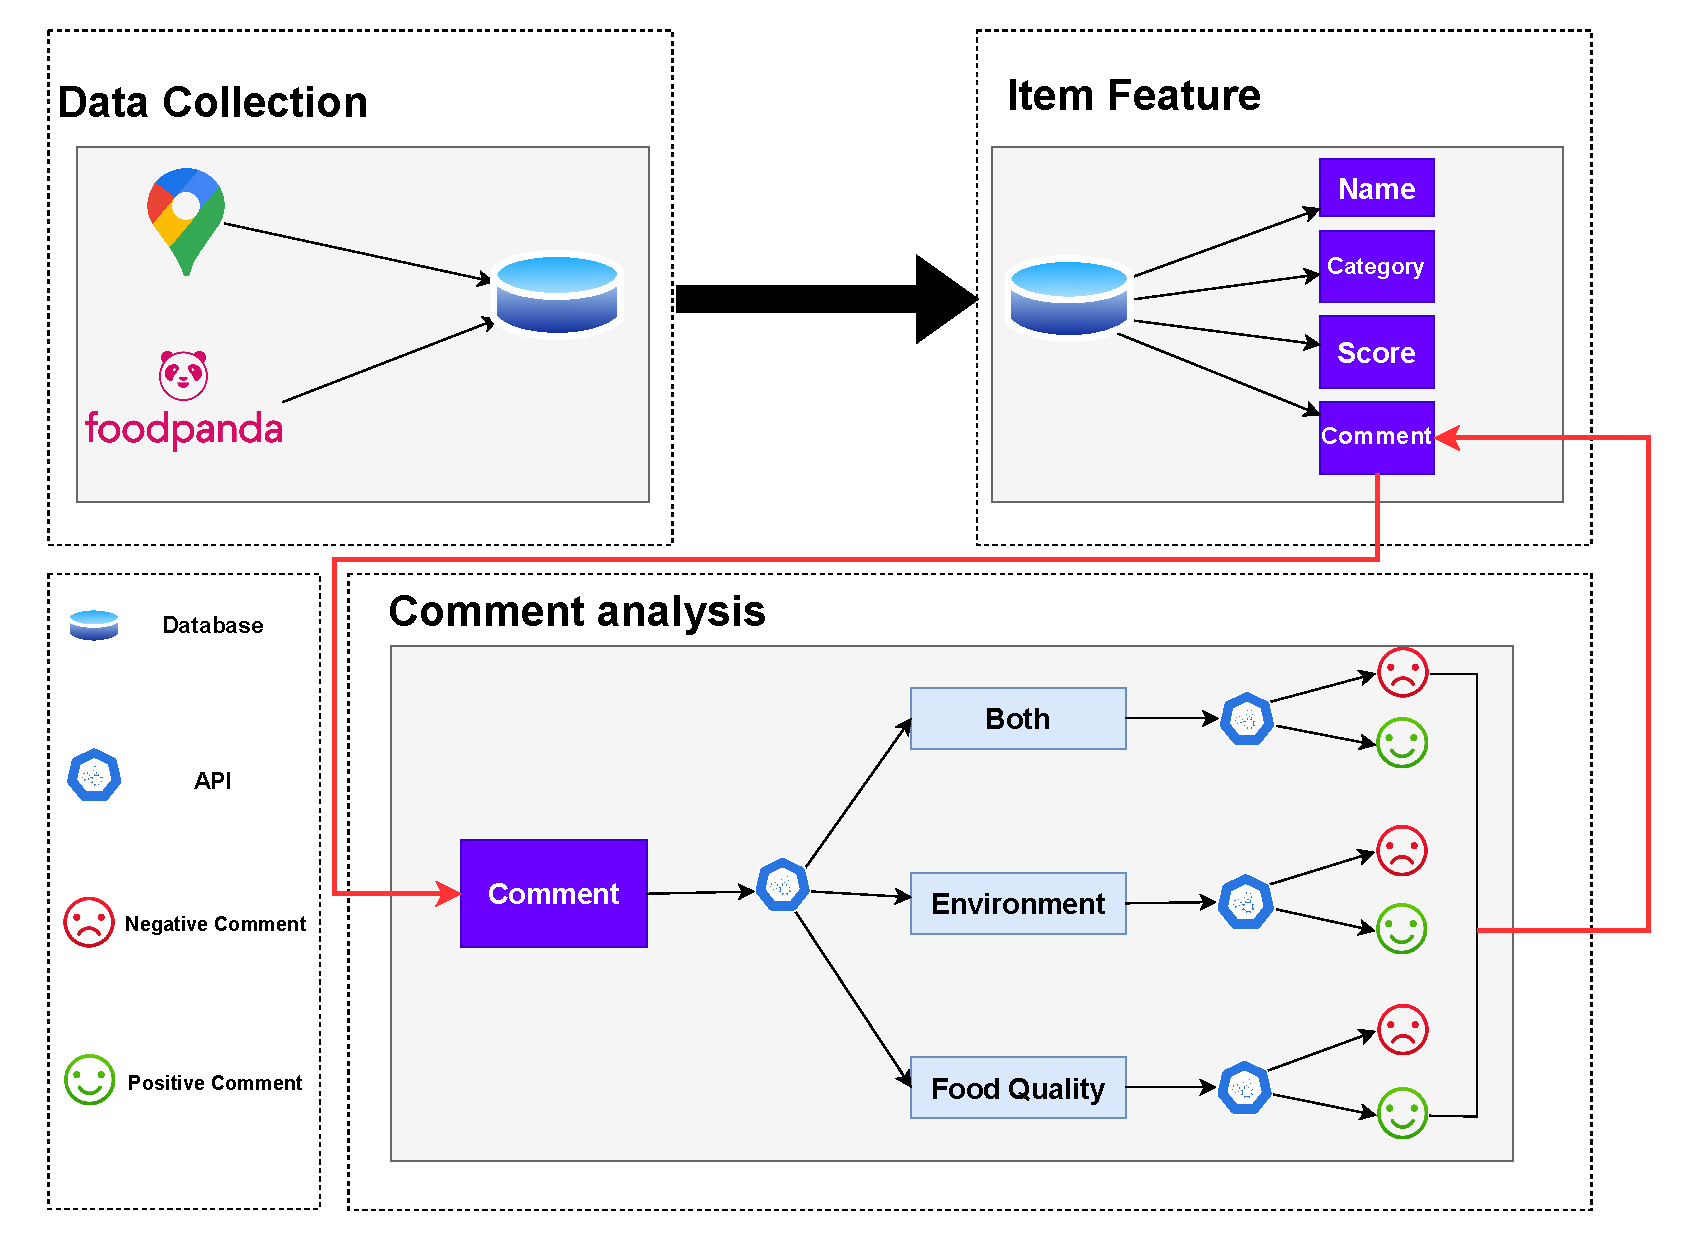
\includegraphics[width=0.5\textwidth]{img/preprocess.pdf}
            \caption{資料前處理架構圖}
            \label{fig-preprocess}
        \end{figure}
        本研究的資料前處理架構如 \xfig{fig-preprocess} 所示,利用爬蟲技術從 Foodpanda 和 Google Maps 獲取餐廳資料。每間餐廳的資料涵蓋了餐廳名稱、餐廳類型、評分以及顧客的評論。由於每家店通常會累積大量的評論,這些評論內容對於描述店家的品質、服務及顧客的體驗具有高度相關性。若將所有評論合併後再丟入 GPT-4 進行分析,可能會因評論主題多樣性導致訊息混雜,進而影響模型的微調(Fine Tuning)效果。當不同主題的評論一起進行訓練時,模型可能難以識別每個特徵的意圖,進而影響結果的精準度。

        為提升模型的針對性,本研究首先將評論依主題分為三類:餐點品質、店內環境氣氛,以及兩者皆有的綜合評價。針對這三類評論,我們分別對每一類進行獨立的 LLM 微調。這種獨立的微調方法有助於每個模型專注於該主題的特徵,避免不同主題之間的訊息干擾。對於餐點品質類評論,模型學習專注於食物的口感、質量及呈現;對於店內環境氣氛的評論,模型則聚焦在用餐氛圍、環境設計及舒適度等描述上;而綜合評價類別則幫助模型掌握顧客的整體體驗。通過分開微調,每個模型能精確捕捉該主題的特徵表現,使得每一類評論的處理結果更具針對性。\color{blue}

        完成初步主題分類與獨立微調後,針對每一類主題中的評論再進行情感分析,以判斷其情感取向為正面或負面。由於共有三種初步主題分類 \( C = \{ c_1, c_2, c_3 \} \),且每個分類中進一步區分為正面(\( P \))與負面(\( N \)),因此共有六種情感分類,定義為集合:
        \begin{equation}
            S = \{ c_1^P, c_1^N, c_2^P, c_2^N, c_3^P, c_3^N \},
            \label{eq-classification}
        \end{equation}
        其中 \( c_1 \) 表示"餐點品質"、\( c_2 \) 表示"店內環境氣氛"、\( c_3 \) 表示"綜合評價";\( P \) 表示該主題分類下的正面情感,\( N \) 表示該主題分類下的負面情感。
        \[
        \mathbf{e}(s) \in \mathbb{R}^d,
        \]
        其中 \( d \) 為嵌入向量的維度。
        
        假設某店家 \( j \) 有 \( n_j \) 條評論,每條評論 \( i \) 的初步主題分類為 \( c_{j,i} \in C \),且每個主題分類對應的權重為 \( w(c_{j,i}) \)。對於第 \( i \) 條評論,其嵌入向量為 \( \mathbf{e}_{j,i} = \mathbf{e}(c_{j,i}) \),權重 \( w(c_{j,i}) \) 根據三種分類具體設定,滿足:
        \begin{equation} 
            w(c) = 
            \begin{cases} 
                w_{1}, & \text{若 } c = c_1, \\ 
                w_{2}, & \text{若 } c = c_2, \\
                w_{3}, & \text{若 } c = c_3, 
            \end{cases} 
            \label{eq-weight} 
        \end{equation}
        其中 \( w_1, w_2, w_3 \) 分別表示三種主題分類的重要性權重。
        本研究對所有評論的嵌入向量進行加權平均:
        \begin{equation} 
            \mathbf{e_j} = \frac{\sum_{i=1}^{n_j} w(c_{j,i}) \cdot \mathbf{e}_{j,i}}{n_j},
            \label{eq-embedding} 
        \end{equation}
        其中 \( \mathbf{e_j} \) 表示店家 \( j \) 涵蓋所有評論所得出之最終的評論嵌入向量。
    \subsection{Dataset}

        
\color{black}